\section{Multiplexed Rotations}
\label{sec:multiplexed-rotations}

Implementing a coherent for-loop over the computational basis states of a register is a common subroutine referred to as multiplexing.
In this section, we discuss the cost and explicit circuit compilation for multiplexed rotations where, for each index of the loop, an arbitrary rotation around the same axis (but different angle) is applied on the same qubit:
\begin{equation}
    \sum_{l=0}^{L - 1} \ket{l} \ket{\phi} \rightarrow \sum_{l=0}^{L - 1} \ket{l} R_a (\alpha_l) \ket{\phi}
\end{equation}

One option for implementing multiplexed rotations is to use the multiplexing structure of Babbush et. al \cite{babbush2018encoding} (Figure 7) where the unitary applied at each index is the explicitly desired rotation.

However, another option, proposed by Möttönen et. al \cite{mottonen2004transformation}, provides a construction specifically for implementing multiplexed rotations.
This construction is only defined for when $L$ is explicitly $2^K$ where $K$ is the number of qubits in the register being multiplexed over.
In this construction, the rotation angles are classically preprocessed based on the Gray code (Eq. 3 of \cite{mottonen2004transformation}):
\begin{equation}
    \begin{bmatrix}
        \theta_{0} \\
        \theta_{1} \\
        \vdots \\
        \theta_{2^K - 1}
    \end{bmatrix} = M \begin{bmatrix}
        \alpha_{0} \\
        \alpha_{1} \\
        \vdots \\
        \alpha_{2^K - 1}
    \end{bmatrix}
\end{equation}
where $M$ is a matrix transformation defined by:
\begin{equation}
    M_{i, j} = 2^{-K} (-1)^{b_{j} . g_{i}}
\end{equation}
where $b_j$ is the binary representation of the integer $j$, $g_i$ is the Gray code representation of the integer $i$, and $b_{j} . g_{i}$ is the bitwise inner product of $b_{j}$ and $g_{i}$.
This construction leads to a cost of $2^K$ arbitrary rotations when implementing \textit{uncontrolled} multiplexed rotations.

It should be noted that rotations by an angle of $\alpha_l = 0$ will likely become nonzero rotations after this classical preproceesing is applied.
This has an impliciation in this work when the coefficients from bosonic ladder operators are applied.
In the main text, we described that the range of the mulitplexor over the occupation of the bosonic mode can be shortened based on the exponents of the creation and annihilation operators since the rotation angle should be zero.
However, these zero-angle rotations will become nonzero when using this construction and therefore will not decrease the cost of implementing the multiplexed rotations.
There are some edge cases where this reduced multiplexing range can reduce the cost, such as when half of the range has zero-valued rotation angles.
We do not include these optimizations in this work as they are highly dependent on the operators in the Hamiltonian being block-encoded.

\begin{figure}
    \centering
    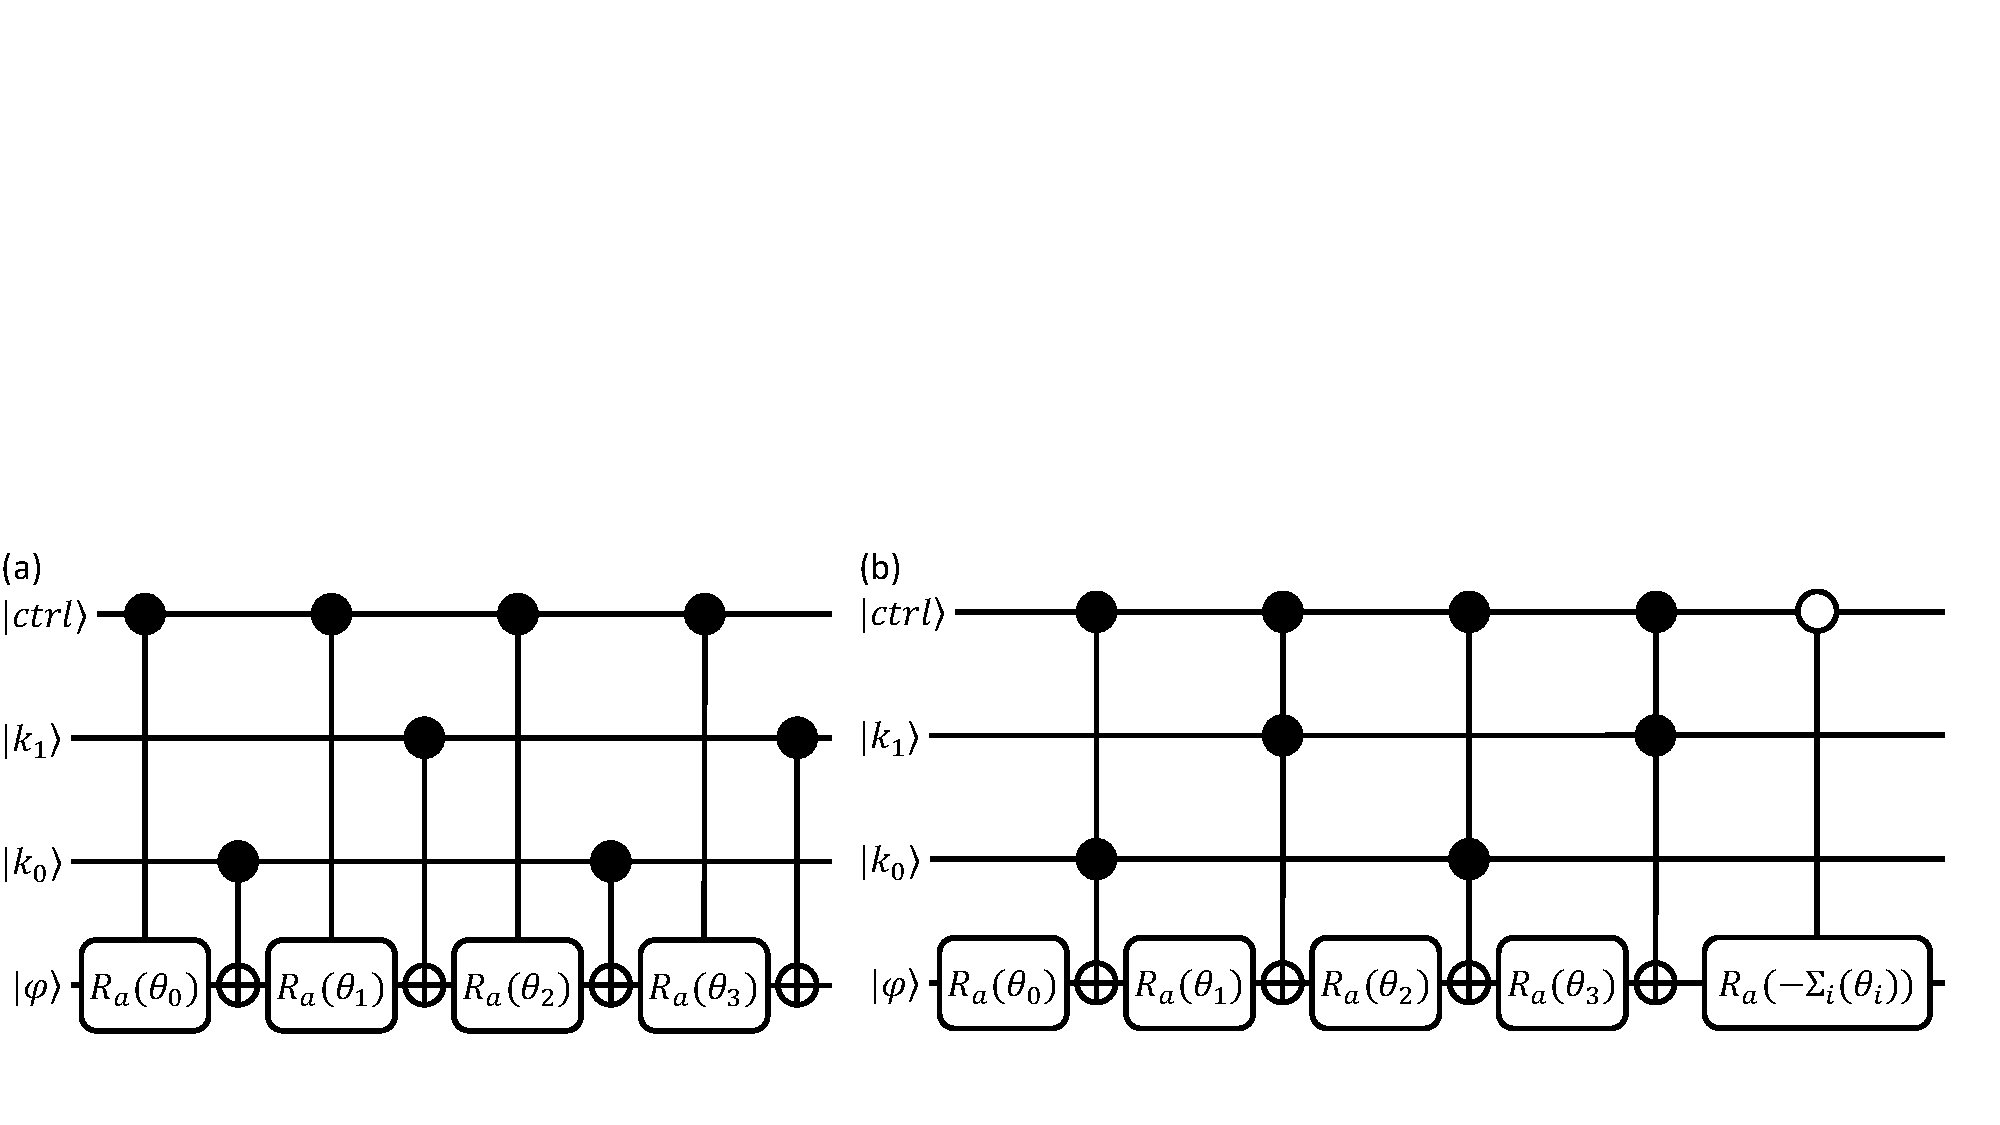
\includegraphics[width=16cm]{figures/controlled-multiplexed-rotations.pdf}
    \caption{
        \textbf{Controlled Multiplexed Rotations}
        Two implementations for controlled multiplexed rotations, building off of the construction presented in \cite{mottonen2004transformation} are shown.
        In subfigure a (left), each arbitrary rotation is simply controlled.
        If the control is off, the CNOT gates will cancel with one another, leaving the quantum state unchanged.
        In subfigure b (right), the arbitrary rotations are left uncontrolled, but the CNOT gates are controlled, promoting them to Toffolis.
        Without the final (controlled) rotation, in the case that the control is off, all rotation gates are applied causing an undesired rotation.
        This undesired rotation can be undone by applying a controlled rotation (controlled on the control being off) of the sum of the angles in the reverse direction.
        This implementation will likely lead to fewer T gates being required assuming that controlling each rotation is more expensive than a Toffoli.
    }
    \label{fig:controlled-multiplexed-rotations}
\end{figure}

Applying the bosonic coefficient rotations, however, requires \textit{controlled} multiplexed rotations.
Naively, this would require controlling each of the arbitrary rotations and allowing the CNOT gates to cancel out with one another when the control is off.
This would then cost $2^K$ \textit{controlled} arbitrary rotations or $2^{K+1}$ uncontrolled arbitrary rotations, since a controlled rotation can be implemented via two uncontrolled rotations and two CNOTs.
An example cirucit diagram for this construction is shown for $K = 2$ in Figure \ref{fig:controlled-multiplexed-rotations}a.

An alternative approach is to control each CNOT gate (promoting each to a Toffoli gate) and leaving each arbitrary rotation uncontrolled.
In this construction, when the control is off none of the Toffolis will fire and the result is an undesired rotation of angle $\sum_{i} (\theta_i)$ applied to the qubit being rotated.
This unwanted rotation can then be undone using one controlled rotation of angle $- \sum_{i} (\theta_i)$ with the condition that the control is off (in the $\ket{0}$ state).
This leads to a cost of $2^K + 2$ rotations and $2^K$ Toffolis (or left/right elbows and one ancilla qubit).
When the number of T gates required for each arbitrary rotation is much larger than $4$ (the number of T gates required for a pair of elbows), this roughly halves the cost of implementing controlled multiplexed rotations as compared to the naive compilation.
An example circuit diagram for this construction is shown for $K = 2$ in Figure \ref{fig:controlled-multiplexed-rotations}b.